\documentclass[]{scrreprt}
\usepackage{amsmath,graphicx}
\usepackage{multirow}
\usepackage{pslatex}
\usepackage{tabularx}
\usepackage{comment}
\usepackage{xspace}
\usepackage{array}

\usepackage{hyperref}

\usepackage{caption}
\DeclareCaptionFont{white}{\color{white}}
\DeclareCaptionFormat{listing}{\colorbox{gray}{\parbox{\textwidth}{#1#2#3}}}

\graphicspath{
{figures/}
}

\newcommand{\uo}{\mbox{UO\textsubscript{2}}\xspace}

\setcounter{secnumdepth}{3}

\newcommand{\si}{\sigma}
\newcommand{\mand}{\ \ \ \mbox{and}\ \ \ }
\newcommand{\pl}{\partial}
\newcommand{\ha}{\mbox{$\frac{1}{2}$}}
\newcommand{\thetac}{\theta^{\mathrm{c}}}
\newcommand{\thetarel}{\theta^{\mathrm{rel}}}
\newcommand{\ep}{\epsilon}
\newcommand{\ga}{\gamma}
\newcommand{\spa}{\ \ \ }
\newcommand{\non}{\nonumber}
\newcommand{\de}{\delta}
\newcommand{\ka}{\kappa}
\newcommand{\la}{\lambda}
\newcommand{\tr}{\mbox{Tr}\,}
\newcommand{\al}{\alpha}
\newcommand{\be}{\beta}
\newcommand{\cd}{\cdot}
\newcommand{\smax}{\sigma_{\mathrm{max}}}
\newcommand{\smid}{\sigma_{\mathrm{mid}}}
\newcommand{\smin}{\sigma_{\mathrm{min}}}

\begin{document}


\title{Capped Mohr-Coulomb Plasticity}
\author{CSIRO}
\maketitle

\tableofcontents


\chapter{Introduction and the yield functions}
\label{yf.chap}

Tensile, or Rankine, plasticity is designed to simulate a material
that fails when the maximum principal stress exceeds the material's tensile
  strength.  Its yield function is therefore
\begin{equation}
  f =  \smax - T \ ,
\end{equation}
where $\smax$ is the maximum\footnote{Often the maximum
  principal stress is denoted by $\smin$.  The code uses the {\tt
    dsymmetricEigenvalues} method of {\tt RankTwoTensor} and this
  orders the eigenvalues from smallest to greatest.} principal
stress (the largest eigenvalue of the stress tensor) and $T$ is the
tensile strength.

One yield function is sufficient because of the definition
$\smin\leq\smid\leq\smax$.  For instance, if during
the return-map process both $\smid$ and $\smax$ exceed
$T$ the corresponding admissible configuration is that both of them
are equal to $T$.  While one yield function is sufficient, it is
convenient to use three yield functions in total:
\begin{eqnarray}
  f_{0} & = & \smax - T \ , \nonumber \\
  f_{1} & = & \smid - T \ , \nonumber \\
  f_{2} & = & \smin - T \ .
  \label{tensile_yfs}
\end{eqnarray}
This is the version used by {\tt TensileStressUpdate}.  These yield
functions have been ordered so that the smoothing creates a surface
that is perpendicular to the $\smax=\smid$ plane, and
that any trial stress with $\smid=\smin$ has an admissible
returned stress.

Similar remarks hold for compressive plasticity.  It yield functions
are
\begin{eqnarray}
  f_{3} & = & -\smin - T_{c} \ , \nonumber \\
  f_{4} & = & -\smid - T_{c} \ , \nonumber \\
  f_{5} & = & -\smax - T_{c}  \ .
  \label{compressive_yfs}
\end{eqnarray}
Here $T_{c}$ is the compressive strength, which is positive for
real-world materials, and must always satisfy $T_{c}>-T$,
otherwise there is no admissible region.

Mohr-Coulomb plasticity simulates a material that undergoes shear
failure if the shear stress exceeds a linear function of the
compressive stress.  Its yield functions are
\begin{eqnarray}
f_{6} & = & \ha (\smax - \smin) +
\ha(\smax+\smin)\sin\phi - C\cos\phi \ , \nonumber \\
f_{7} & = & \ha (\smid - \smin) +
\ha(\smid+\smin)\sin\phi - C\cos\phi \ , \nonumber \\
f_{8} & = & \ha (\smax - \smid) +
\ha(\smax+\smid)\sin\phi - C\cos\phi \ , \nonumber \\
f_{9} & = & \ha (\smid - \smax) +
\ha(\smid+\smax)\sin\phi - C\cos\phi \ , \nonumber \\
f_{10} & = & \ha (\smin - \smid) +
\ha(\smin+\smid)\sin\phi - C\cos\phi \ , \nonumber \\
f_{11} & = & \ha (\smin - \smax) +
\ha(\smin+\smax)\sin\phi - C\cos\phi \ .
\label{mc_fs}
\end{eqnarray}
Here $C$ is the cohesion and $\phi$ is the friction angle.  Once
again, the yield functions have been ordered optimally.

Equations~(\ref{tensile_yfs}), (\ref{compressive_yfs})
and~(\ref{mc_fs}) define the yield functions of Capped Mohr Coulomb plasticity.

The return-map algorithm first rotates $\sigma$ from the physical
frame to the
principal-stress frame (where $\sigma = \mbox{diag}(\smin, \smid,
\smax)$).  The rotation matrices used are assumed not to change
during the return-map process: only $\smin$, $\smid$ and
$\smax$ change.  Therefore, at the end of the
return-map process these rotation matrices may be used to find the
final stress in the physical frame.

The 12 yield functions are smoothed using the method encoded in {\tt
  MultiParameterPlasticityStressUpdate}.  An example is shown
Figures~\ref{cmc_3D.fig} and~\ref{cmc_oct.fig}.
Figure~\ref{cmc_oct.fig} shows slices of the yield surface at various
values of the mean stress (that is, on various octahedral planes), and
the hexagonal-pyramid and triangular-pyramid nature of the yield
surface is evident.  The slices taken near the tip and the base
highlight: (1) the smoothing; (2) that the smoothing is unsymmetric.

The unsymmetric nature of the
yield surface only occurs near the tip and base region where the smoothing
mixes the three yield surfaces.  For instance, the black line in
Figure~\ref{cmc_oct.fig} is symmetric, while the red
lines are unsymmetric.  The amount of asymmetry is small, but it is
evident that the red curve is not concentric with the remainder of the
curves shown in Figure~\ref{cmc_oct.fig}.  The order of the yield
functions in Eqn~(\ref{tensile_yfs}), (\ref{compressive_yfs})
and~(\ref{mc_fs}) have been chosen so that: at the tip the curves
intersect the $\smax=\smid$ line at $90^{\circ}$, but not
on the $\smid=\smin$ line; at the base the curves
intersect the $\smid=\smin$ line at $90^{\circ}$, but not
on the $\smax=\smid$ line.  The
asymmetry does not affect MOOSE's convergence, and of course it is
physically irrelevant (since there is no one ``correct'' smoothed
yield surface).

\begin{figure}[htb]
  \begin{center}
    \begin{tabular}{ll}
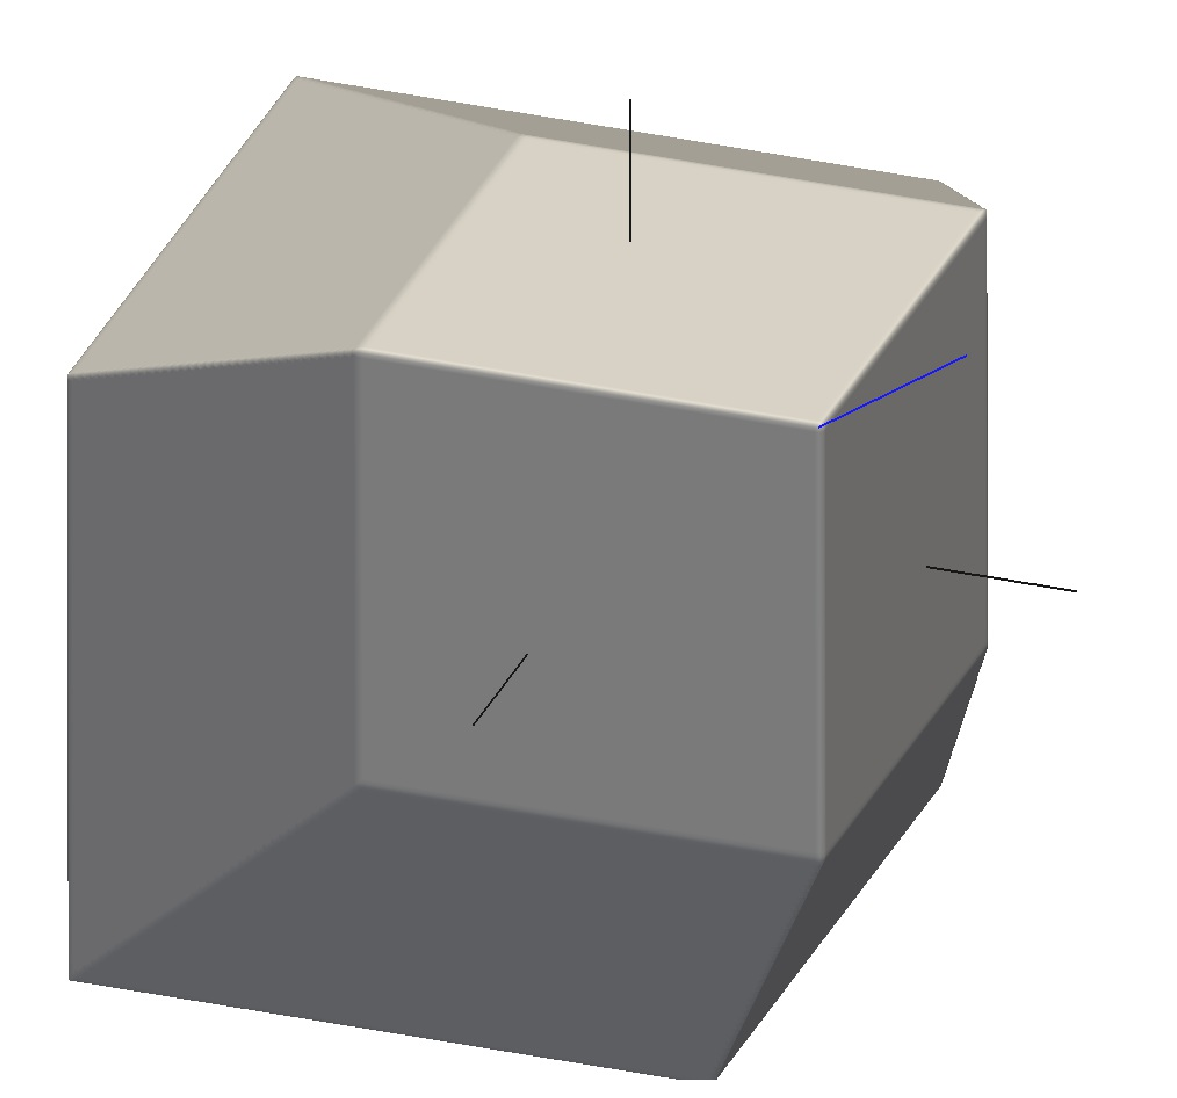
\includegraphics[width=6cm]{capped_mc_3D_unsmoothed.eps} &
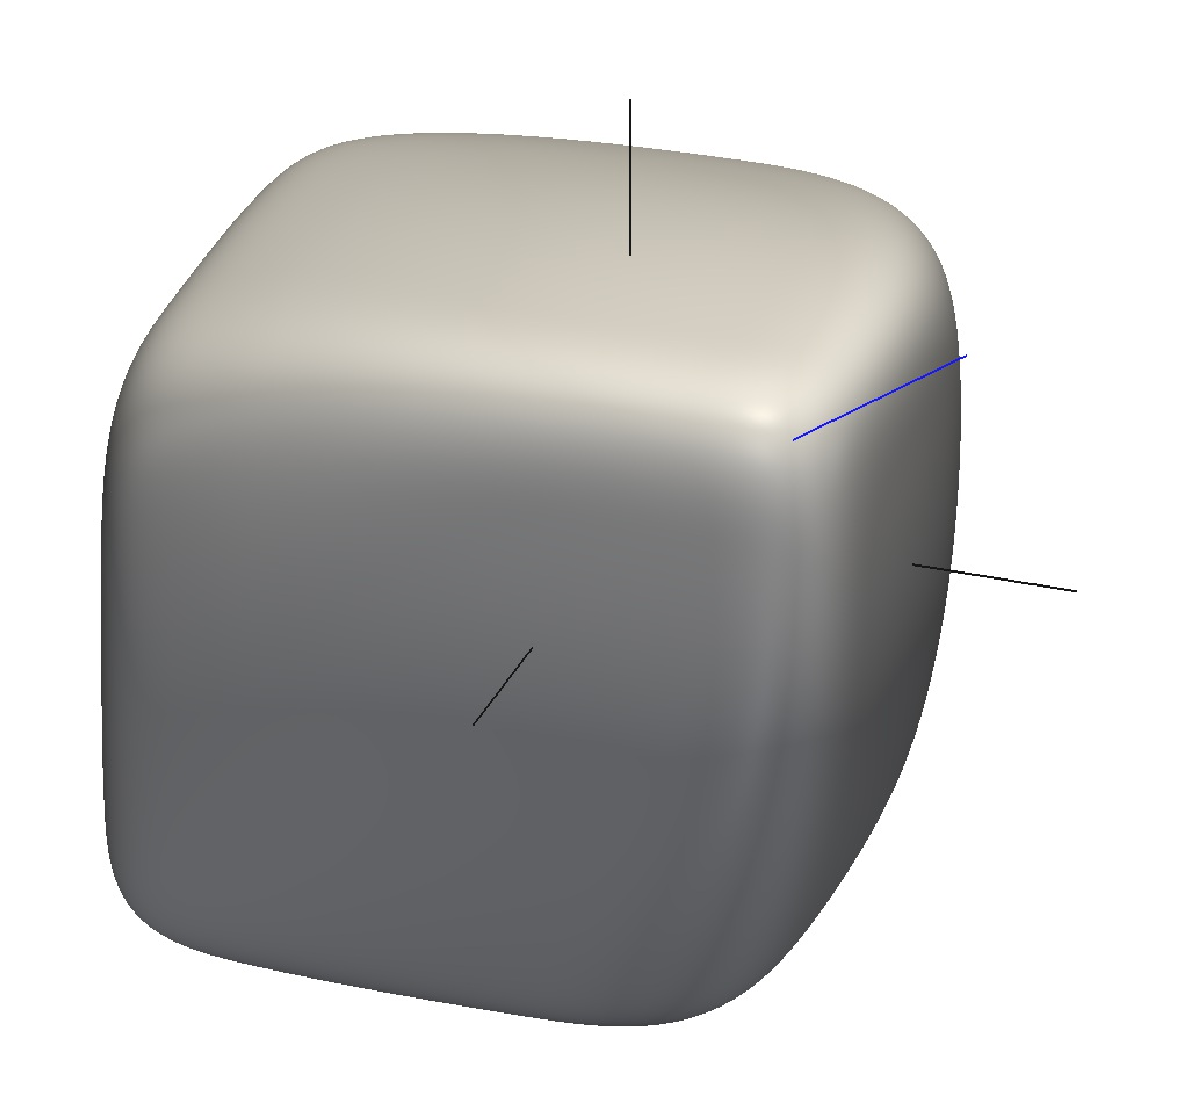
\includegraphics[width=6cm]{capped_mc_3D_smoothed.eps}
    \end{tabular}
\caption{Left: the unsmoothed yield surface of capped Mohr-Coulomb
  plasticity, which is a hexagonal pyramid, capped with a trianglar
  pyramid at its tip and base (the base is not visible in this
  picture).  Right: a smoothed version.  The principal stress
  directions are shown with black lines, and the mean stress direction
  is shown with a blue line.  In these pictures $C=3$,
  $\phi=30^{\circ}$, $T=0.4$, $T_{c}=0.7$, and the smoothing solerance
  is $0.2$.}
\label{cmc_3D.fig}
\end{center}
\end{figure}

\begin{figure}[htb]
  \begin{center}
    \begin{tabular}{ll}
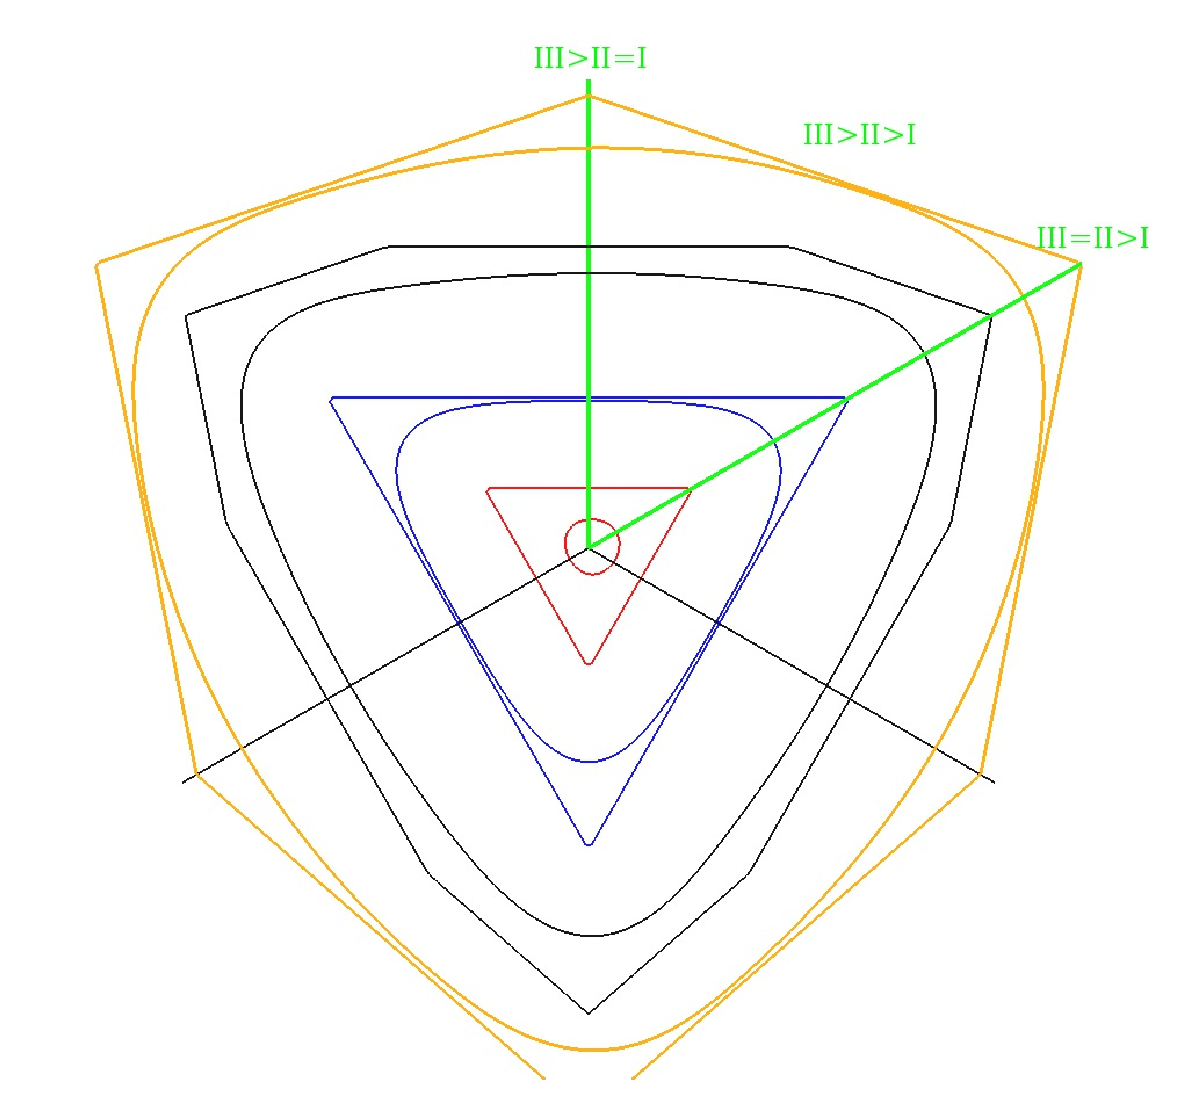
\includegraphics[width=6cm]{capped_mc_2D_tip.eps} &
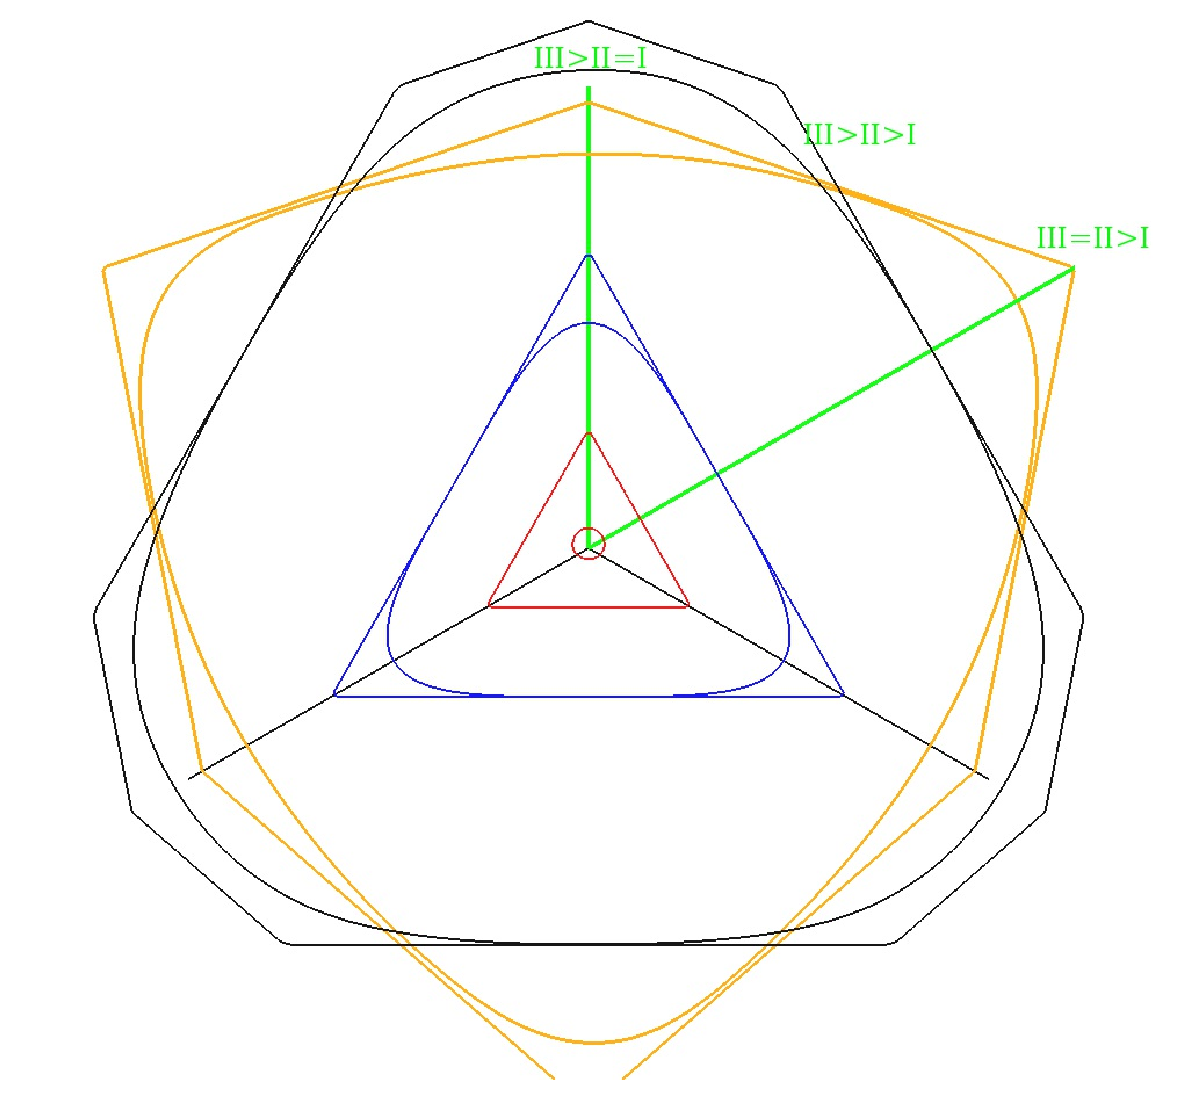
\includegraphics[width=6cm]{capped_mc_2D_base.eps}
    \end{tabular}
\caption{Slices of the unsmoothed and smoothed yield functions at
  various value of mean stress.  The viewer is looking along the line
  of increasing mean stress in these figures.  Left: the orange lines show the
  Mohr-Coulomb hexagon; the black lines show this being truncated by
  the tensile tip; blue lines show the tensile triangle; red lines
  show the yield surface near the tip.  Right: the similar situation
  near the compressive base.  The whole octahedral plane is shown in this figure, but
  only one sextant is physical, which is indicated by the solid green
  lines.  In this figure $III$ represents $\smax$, $II$ represents $\smid$ and $I$ represents $\smin$.}
\label{cmc_oct.fig}
\end{center}
\end{figure}


\chapter{Flow rules and hardening}

The flow potentials for the
tensile and compressive parts are associative, while the flow
potentials for the Mohr-Coulomb parts are nonassociative.  The flow
potentials are:
\begin{eqnarray}
  g_{0} & = & \smax - T \ , \nonumber \\
  g_{1} & = & \smid - T \ , \nonumber \\
  g_{2} & = & \smin - T \ , \nonumber \\
  g_{3} & = & -\smin - T_{c} \ , \nonumber \\
  g_{4} & = & -\smid - T_{c} \ , \nonumber \\
  g_{5} & = & -\smax - T_{c} \ , \nonumber \\
g_{6} & = & \ha (\smax - \smin) +
\ha(\smax+\smin)\sin\psi - C\cos\psi \ , \nonumber \\
g_{7} & = & \ha (\smid - \smin) +
\ha(\smid+\smin)\sin\psi - C\cos\psi \ , \nonumber \\
g_{8} & = & \ha (\smax - \smid) +
\ha(\smax+\smid)\sin\psi - C\cos\psi \ , \nonumber \\
g_{9} & = & \ha (\smid - \smax) +
\ha(\smid+\smax)\sin\psi - C\cos\psi \ , \nonumber \\
g_{10} & = & \ha (\smin - \smid) +
\ha(\smin+\smid)\sin\psi - C\cos\psi \ , \nonumber \\
g_{11} & = & \ha (\smin - \smax) +
\ha(\smin+\smax)\sin\psi - C\cos\psi \ .
\end{eqnarray}
Here $\psi$ is the dilation angle.

The flow rules are
\begin{equation}
  s_{a} = s_{a}^{\mathrm{trial}} - \ga E_{ab} \frac{\partial
    g}{\partial s_{a}} \ ,
  \label{eqn.flow.rules}
\end{equation}
where $s_{a}=\{\smin, \smid, \smax\}$ and
\begin{equation}
  E_{ab} = \frac{\partial s_{a}}{\partial \sigma_{ij}} E_{ijkl}
  \frac{\partial s_{b}}{\partial \sigma_{kl}} \ .
\end{equation}
In this equation $E_{ijkl}$ is the elasticity tensor.

An assumption
that is made in {\tt  MultiParameterPlasticityStressUpdate} is that
$E_{ab}$ is independent of the stress parameters, $s_{a}$ and the
internal variables.  In this case\footnote{Special precautions are
  taken when the eigenvalues are equal, as described in {\tt RankTwoTensor}.}
\begin{equation}
  \frac{\partial s_{a}}{\partial \sigma_{ij}} = v_{i}^{a}v_{j}^{a} \ ,
\end{equation}
where $v^{a}$ is the eigenvector corresponding to the eigenvalue
$s^{a}$ (of the stress tensor) and there is no sum over $a$ on the
right-hand side.  Recall that the eigenvectors are fixed during the
return-map process, so the RHS is fixed, meaning that $E_{ab}$ is
indeed independent of the stress parameters.  Also recall that the
eigenvectors induce a rotation (to the principal-stress frame), so
assuming that $E_{ijkl}$ is isotropic
\begin{equation}
  E_{ab} = E_{aabb} \ .
\end{equation}
The assumption of isotropy is appropriate for this type of isotropic
plasticity.

It is assumed that there are two internal parameters.  Note that the
definition of internal parameters is motivated by thought experiments
or by real experiments, and as such, the following definitions might
not suit your needs.  It is a small job to produce a new version of
{\tt CappedMohrCoulomb} that incorporates different internal parameters.

The ``shear''
internal parameter is $i_{0}$, while the ``tensile'' internal
parameter is $i_{1}$.  It is assumed that
\begin{eqnarray}
  C & = & C(i_{0}) \ , \nonumber \\
  \phi & = & \phi(i_{0}) \ , \nonumber \\
  \psi & = & \psi(i_{0}) \ , \nonumber \\
  T & = & T(i_{1}) \ , \nonumber \\
  T_{c} & = & T_{c}(i_{1}) \ .
\end{eqnarray}
The evolution of $i_{0}$ and $i_{1}$ is motivated by first considering
a pure shear failure.  I would like $i_{1}$ to be unchanged in pure shear.  A
pure shear failure implies
\begin{eqnarray}
  0 & = & f = \ha (\smax - \smin) + \ha (\smax +
  \smin)\sin\phi - C \cos\phi \ , \nonumber \\
  \smax & = & \smax^{\mathrm{trial}} -
  \gamma_{\mathrm{shear}} E_{22}(\ha + \ha\sin\psi) -
  \gamma_{\mathrm{shear}} E_{20}(-\ha + \ha\sin\psi) \ , \nonumber \\
  \smin & = & \smin^{\mathrm{trial}} -
  \gamma_{\mathrm{shear}} E_{00}(-\ha + \ha\sin\psi) -
  \gamma_{\mathrm{shear}} E_{02}(\ha + \ha\sin\psi) \ .
\end{eqnarray}
The first equation is the yield function and the other equations are
the flow rules.   Combining the last 2 equations yields
\begin{equation}
  \gamma_{\mathrm{shear}} = \frac{(\smax^{\mathrm{trial}} -
    \smin^{\mathrm{trial}}) - (\smax - \smin)}{E_{22}
    - E_{20}}
\end{equation}
It is assumed that the shear internal parameter evolves according to
\begin{equation}
  i_{0} = i_{0}^{\mathrm{old}} + \ga_{\mathrm{shear}} \ .
\end{equation}
Finally, before considering the tensile failure, note that the
equations imply
\begin{equation}
  (\smax^{\mathrm{trial}} + \smin^{\mathrm{trial}})  - (\smax + \smin) =
  \gamma_{\mathrm{shear}} \left(E_{22} + E_{20} \right)\sin\psi \ .
  \label{eqn.shear.correct}
\end{equation}

Now consider a pure tensile failure.  The equations to solve are
\begin{eqnarray}
  0 & = & f = \smax - T \ , \nonumber \\
  \smax & = & \smax^{\mathrm{trial}} -
  \gamma_{\mathrm{tensile}}E_{22} \ .
\end{eqnarray}
The flow rule for $\smin$ is $\smin = \smin^{\mathrm{trial}} -
\gamma_{\mathrm{tensile}}E_{20} = \smin^{\mathrm{trial}} -
\gamma_{\mathrm{tensile}}\mbox{$\frac{\nu}{1-\nu}$}E_{22}$, where
$\nu$ is the Poisson's ratio.  Solving these equations yields
\begin{equation}
  \gamma_{\mathrm{tensile}} = \frac{\smax^{\mathrm{trial}} -
    \smax}{E_{22}} = (1 - \nu) \frac{(\smax^{\mathrm{trial}} +
    \smin^{\mathrm{trial}}) - (\smax + \smin)}{E_{22}} \ .
\end{equation}
The final expression is used.  To motivate this, consider a pure
compressive failure.  The equations to solve are
\begin{eqnarray}
  0 & = & f = -\smin - T_{c} \ , \nonumber \\
  \smin & = & \smin^{\mathrm{trial}} +
  \gamma_{\mathrm{compressive}}E_{00} \ .
\end{eqnarray}
The flow rule for $\smax$ is $\smax = \smax^{\mathrm{trial}} +
\gamma_{\mathrm{compressive}}\mbox{$\frac{\nu}{1-\nu}$}E_{00}$, where
$\nu$ is the Poisson's ratio.  Solving these equations yields
\begin{equation}
  \gamma_{\mathrm{compressive}} = - (1 - \nu) \frac{(\smax^{\mathrm{trial}} +
    \smin^{\mathrm{trial}}) - (\smax + \smin)}{E_{00}} \ .
\end{equation}
Note that $\gamma_{\mathrm{compressive}} =
-\gamma_{\mathrm{tensile}}$.  This means that when these expressions for
the plastic multipliers are used a compressive failure following a
tensile failure can cause the tensile internal parameter to reduce,
which is physically appealing.

The evolution of the tensile internal parameter is assumed to obey
\begin{equation}
  i_{1} = i_{1}^{\mathrm{old}} + (1 -
  \nu)\frac{(\smax^{\mathrm{trial}} + \smin^{\mathrm{trial}}) -
    (\smax + \smin) - \gamma_{\mathrm{shear}} \left(E_{22} + E_{20}\right)\sin\psi}{E_{22}} \ .
\end{equation}
The reason for the final term involving $\gamma_{\mathrm{shear}}$ is
to ensure that no increment of the tensile internal parameter occurs
during pure shear failure --- see Eqn~(\ref{eqn.shear.correct}).
However, the above definitions mean that during pure tensile failure,
the shear internal parameter will change.

\chapter{Technical discussions}

\section{Unknowns and the convergence criterion}
The return-map problem involves solving the four equations: $f=0$ (smoothed yield function
should be zero) and the flow equations~(\ref{eqn.flow.rules}).  The
unknowns are the 3 stress parameters $s_{a}=\{\smin, \smid,
\smax\}$ and the plasticity multiplier $\ga$.  Actually, to
make the units consistent the algorithm uses $\ga E_{22}$ instead of
simply $\ga$.  Convergence
is deemed to be achieved when the sum of squares of the residuals of
these 4 equations is less than a user-defined tolerance.

\section{Iterative procedure and initial guesses}
A Newton-Raphson process is used, along with a cubic line-search.  The
process may be initialised with the solution that is correct for
perfect plasticity (no hardening) and no smoothing, if the user
desires.  Smoothing adds nonlinearities, so this initial guess will
not always be the exact answer. For hardening, it is not
always advantageous to initialise the Newton-Raphson process in this
way, as the yield surfaces can move dramatically during the return
process.

\section{Substepping the strain increments}
Because of the difficulties encountered during the Newton-Raphson
process during rapidly hardening/softening moduli, it is possible to
subdivide the applied strain increment, $\delta\epsilon$, into smaller
substeps, and do multiple return-map processes.  The final returned configuration may then
be dependent on the number of substeps.  While this is simply
illustrating the non-uniqueness of plasticity problems, in my
experience it does adversely affect MOOSE's nonlinear convergence as
some Residual calculations will take more substeps than other Residual
calculations: in effect this is reducing the accuracy of the Jacobian.

\section{The consistent tangent operator}
MOOSE's Jacobian depends on the derivative
\begin{equation}
H_{ijkl} = \frac{\delta\sigma_{ij}}{\delta \epsilon_{kl}} \ .
\end{equation}
The quantity $H$ is called the consistent tangent operator.  For pure
elasticity it is simply the elastic tensor, $E$, but it is more
complicated for plasticity.  Note that a small $\delta\epsilon_{kl}$
simply changes $\delta\sigma^{\mathrm{trial}}$, so $H$ is capturing the
change of the returned stress ($\delta\sigma$) with respect to a
change in the trial stress ($\delta\sigma^{\mathrm{trial}}$).  In formulae:
\begin{equation}
  H_{ijkl} = \frac{\delta\sigma_{ij}}{\delta
    \sigma_{mn}^{\mathrm{trial}}}
  \frac{\delta\sigma_{mn}^{\mathrm{trial}}}{\delta\epsilon_{kl}} =\frac{\delta\sigma_{ij}}{\delta
    \sigma_{mn}^{\mathrm{trial}}} E_{mnkl} \ .
\end{equation}

In the case at hand,
\begin{equation}
  \sigma_{ij} = \sum_{a}R_{ia}s_{a}R_{aj}^{\mathrm{T}} \ .
\end{equation}
In this formula $\sigma_{ij}$ is the returned stress, $s_{a}$ are the
returned stress parameters (eigenvalues), and $R$ is the rotation
matrix, defined through the eigenvectors, $v^{a}$ ($a=1,2,3$) of the
trial stress:
\begin{equation}
  R_{ia} = v^{a}_{i} \ .
\end{equation}
The three eigenvectors remain unchanged during the return-map
process.  However, of course they change under a change in
$\sigma^{\mathrm{trial}}$.  The relevant formulae are
\begin{eqnarray}
  \frac{\delta s_{a}^{\mathrm{trial}}}{\delta
    \sigma_{kl}^{\mathrm{trial}}} & = & v^{a}_{i}v^{a}_{j} \ , \\
  \frac{\delta v^{a}_{i}}{\delta \sigma_{kl}^{\mathrm{trial}}} & = &
  \sum_{b\neq a}\frac{v_{i}^{b}(v_{k}^{b}v_{l}^{a} +
    v_{l}^{b}v_{k}^{a})}{2(s_{a}-s_{b})} \ .
\end{eqnarray}
On the RHS of these equations there is no sum over $a$.

The final piece of information is
\begin{equation}
  \frac{\delta s_{b}}{\delta s_{a}^{\mathrm{trial}}} \ .
\end{equation}
{\tt MultiParameterPlasticityStressUpdate} computes this after each
Newton step, for any aribtrary plasticity model.

The nontrivial part to the consistent tangent operator is therefore
\begin{equation}
  \frac{\delta \sigma_{ij}}{\delta\sigma_{mn}^{\mathrm{trial}}} =
\sum_{a}  \frac{\delta
    R_{ia}}{\delta\sigma_{mn}^{\mathrm{trial}}}s_{a}R_{aj}^{\mathrm{T}}
  + \sum_{a}\sum_{b} R_{ia}\frac{\delta s_{a}}{\delta s_{b}^{\mathrm{trial}}}
  \frac{\delta s_{b}^{\mathrm{trial}}}{\delta
    \sigma_{mn}^{\mathrm{trial}}}R_{aj}^{\mathrm{T}} +
  \sum_{a} R_{ia}s_{a}\frac{\delta
    R_{aj}^{\mathrm{T}}}{\delta\sigma_{mn}^{\mathrm{trial}}} \ .
\end{equation}
All the components of this equation have been provided above.


\chapter{Tests}

The test suite consists of many tests of {\tt
  CappedMohrCoulombStressUpdate}.  This Chapter describes a few of
these.

\section{The tensile yield surface}

Consider the tip of the tensile yield surface shown in
Figure~\ref{small_deform_5_6_7.fig}.  Repeated deformations may be
applied to a single element in order to cause tensile failure, and by
recording the returned stresses, the yield surface may be mapped out.
Figure~\ref{small_deform_5_6_7.fig} shows that MOOSE produces the
expected result.  The tests are {\tt small\_deform5}, {\tt
  small\_deform6} and {\tt small\_deform7}.

\begin{figure}[htb]
  \begin{center}
    \begin{tabular}{ll}
      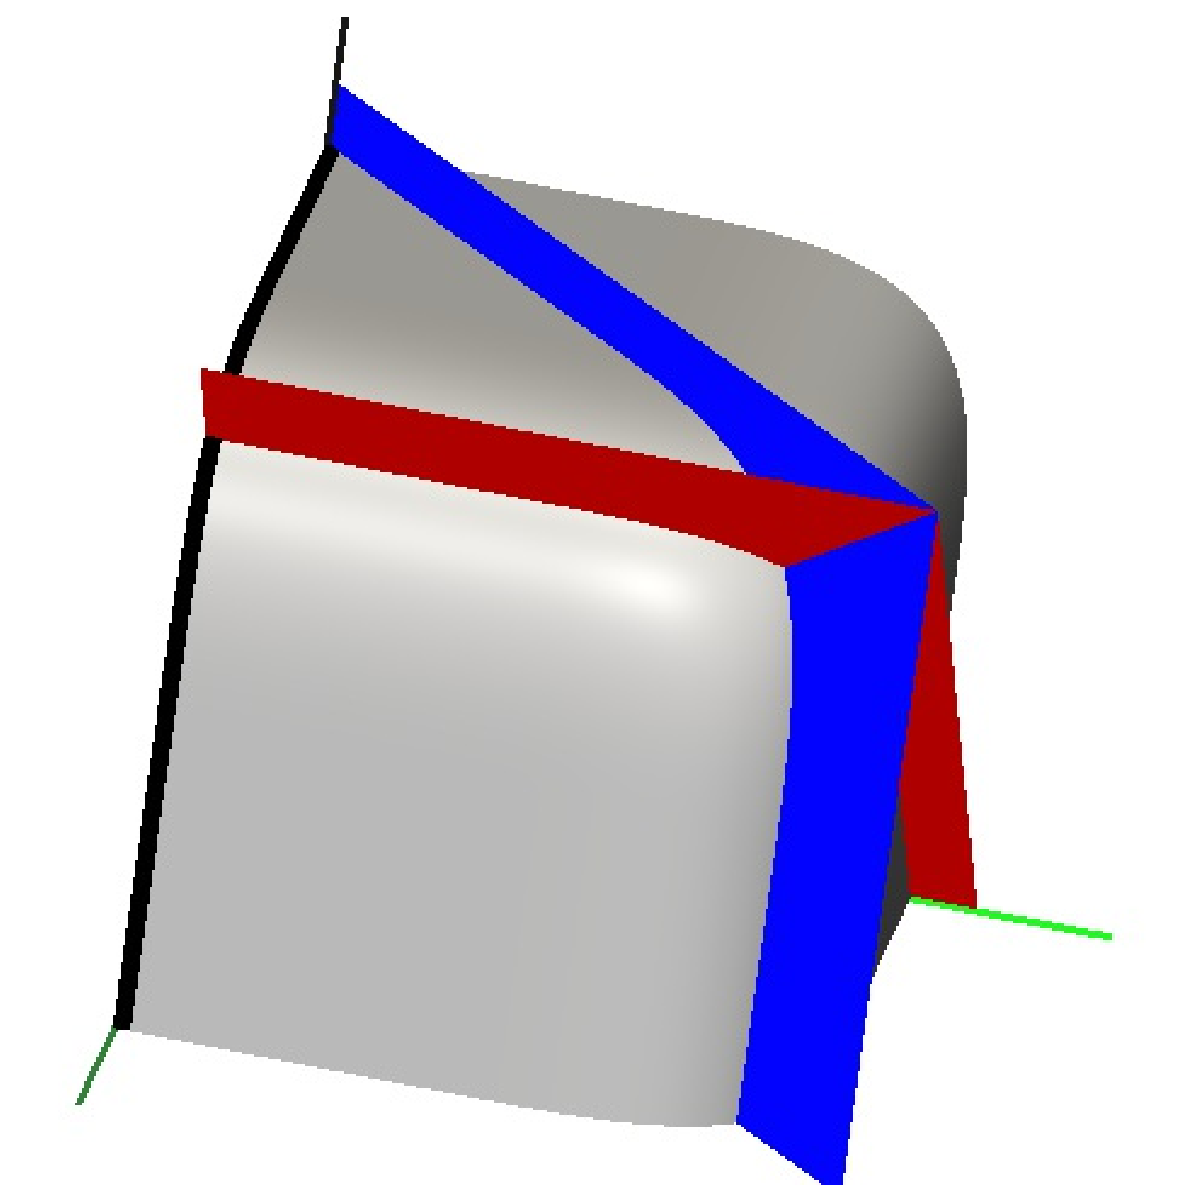
\includegraphics[width=6cm]{tensile_with_planes.eps} &
      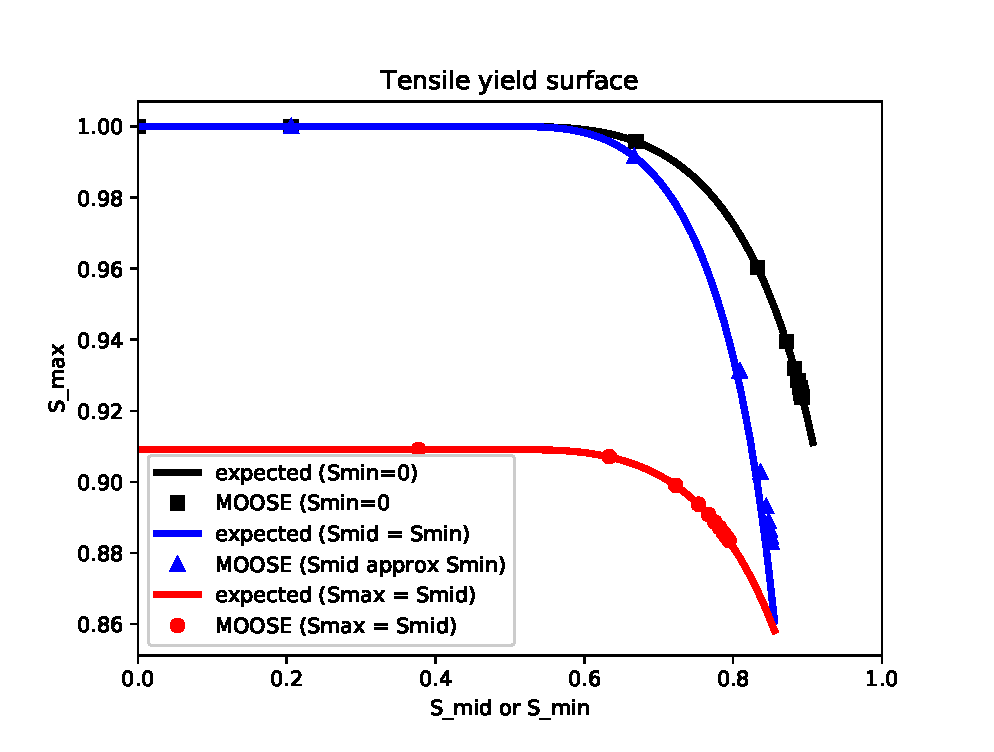
\includegraphics[width=8cm]{small_deform_5_6_7.eps}
    \end{tabular}
\caption{The tip of the tensile yield surface.  This surface has $T=1$
  and the smoothing parameter is 0.5.  The
  principal stress axes are shown in black ($\smax$), dark green
  ($\smid$) and light green ($\smin$).  The wedge-shaped region
  defined by the planes is the physical region where
  $\smax\geq\smid\geq\smin$.  The blue plane is $\smid=\smin$, which
  is a Lode angle of $-30^{\circ}$.  The red plane is $\smax=\smid$,
  which is a Lode angle of $30^{\circ}$.  The black curve has
  $\smin=0$.  The right figure shows plots of the yield surface along
  these curves (with the same colour scheme) demonstrating that MOOSE
  produces the expected result.  There is a tiny discrepancy in the
  blue ($\smid=\smin$) result: this is because the deformations
  applied in the test only produce the approximate result
  $\smid\approx\smin$, so the MOOSE results don't lie exactly on the
  blue plane, but slightly off it.}
\label{small_deform_5_6_7.fig}
\end{center}
\end{figure}

\section{The compressive yield surface}

Consider the tip of the compressive yield surface shown in
Figure~\ref{small_deform_15_16_17.fig}.  Repeated deformations may be
applied to a single element in order to cause compressive failure, and by
recording the returned stresses, the yield surface may be mapped out.
Figure~\ref{small_deform_15_16_17.fig} shows that MOOSE produces the
expected result.  The tests are {\tt small\_deform15}, {\tt
  small\_deform16} and {\tt small\_deform17}.

\begin{figure}[htb]
  \begin{center}
    \begin{tabular}{ll}
      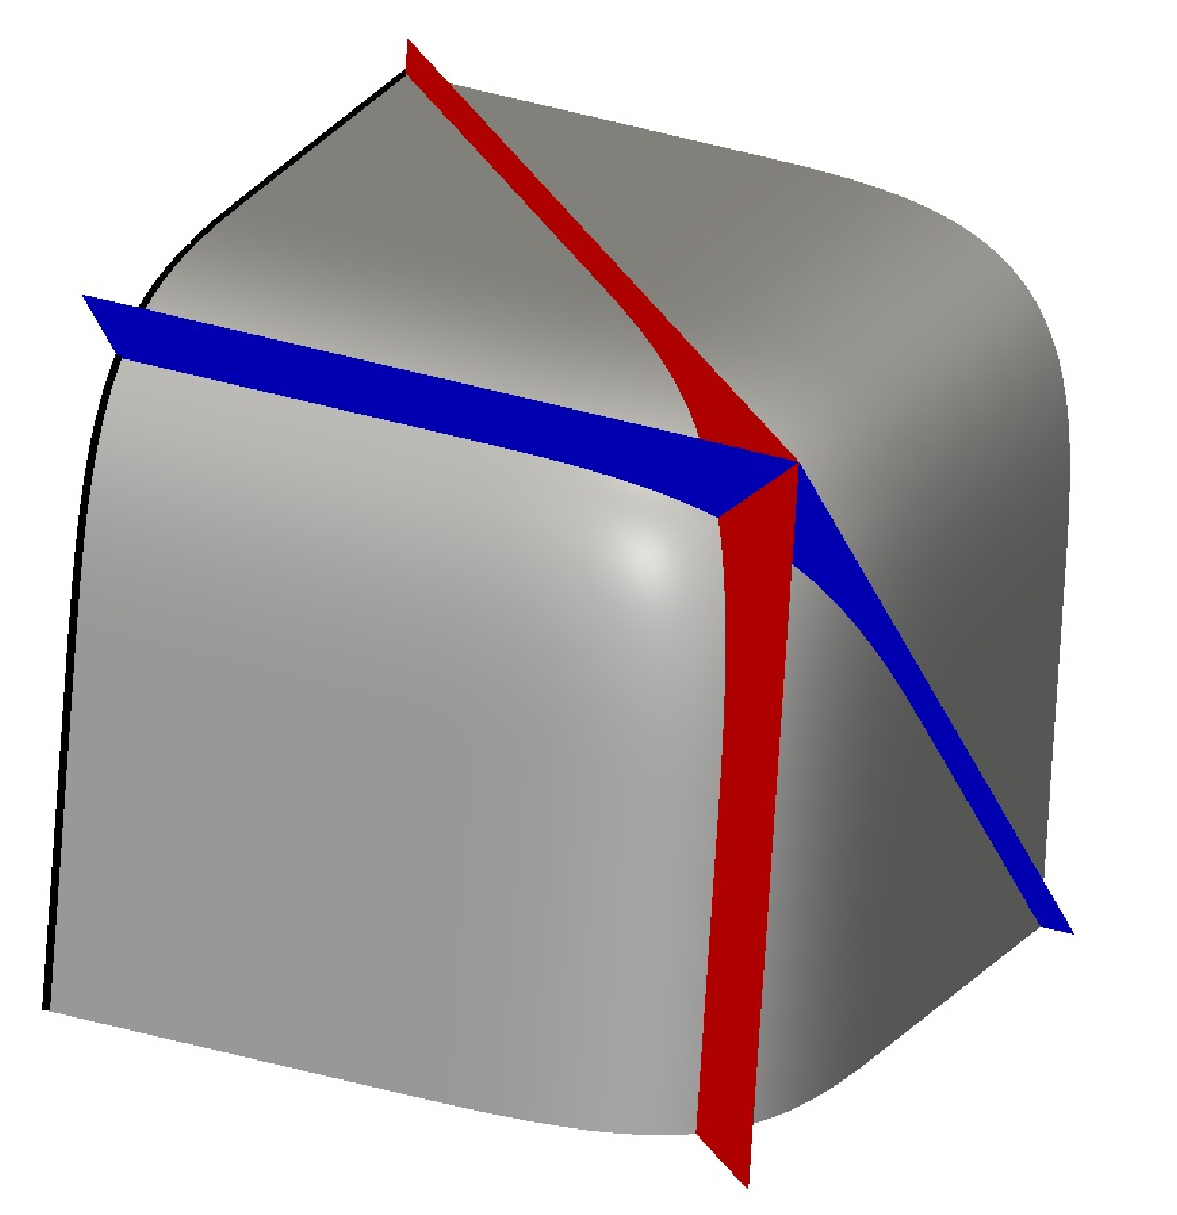
\includegraphics[width=6cm]{compressive_with_planes.eps} &
      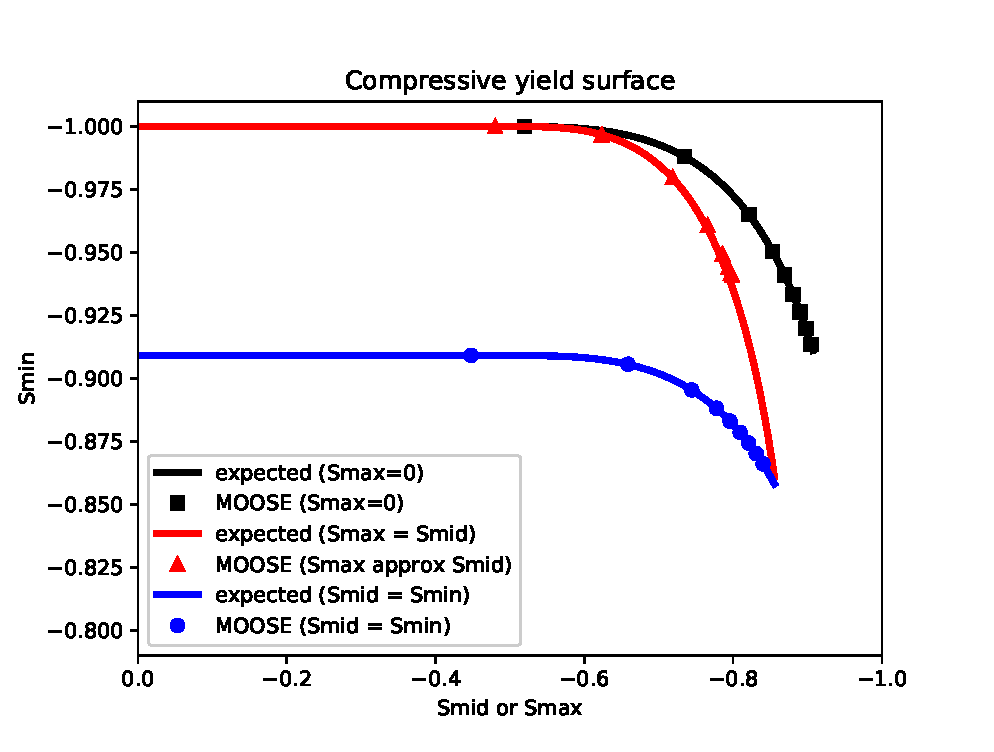
\includegraphics[width=8cm]{small_deform_15_16_17.eps}
    \end{tabular}
\caption{The tip of the compressive yield surface (this view has
  opposite orientation to Figure~\ref{small_deform_15_16_17.fig}).
  This surface has $T_{c}=1$ and the smoothing parameter is 0.5.  The
  wedge-shaped region defined by the planes is the physical region
  where $\smax\geq\smid\geq\smin$.  The blue plane is $\smid=\smin$,
  which is a Lode angle of $-30^{\circ}$.  The red plane is
  $\smax=\smid$, which is a Lode angle of $30^{\circ}$.  The black
  curve has $\smax=0$.  The right figure shows plots of the yield
  surface along these curves (with the same colour scheme)
  demonstrating that MOOSE produces the expected result.  There is a
  tiny discrepancy in the red ($\smax=\smid$) result: this is because
  the deformations applied in the test only produce the approximate
  result $\smax\approx\smid$, so the MOOSE results don't lie exactly
  on the blue plane, but slightly off it.}
\label{small_deform_15_16_17.fig}
\end{center}
\end{figure}


\section{The Mohr-Coulomb yield surface on the octahedral plane}

Consider the slice of the Mohr-Coulomb yield surface shown in
Figure~\ref{mc_octahedral_plane.fig}, where the mean stress is zero:
$\tr\sigma = 0$.  Repeated deformations may be applied to a single element in order to
cause shear failure, and by recording the returned stresses, the yield
surface may be mapped out.   The result is shown in
Figure~\ref{mc_octahedral_plane.fig}.  The test is {\tt small\_deform21}.

\begin{figure}[htb]
  \begin{center}
    \begin{tabular}{ll}
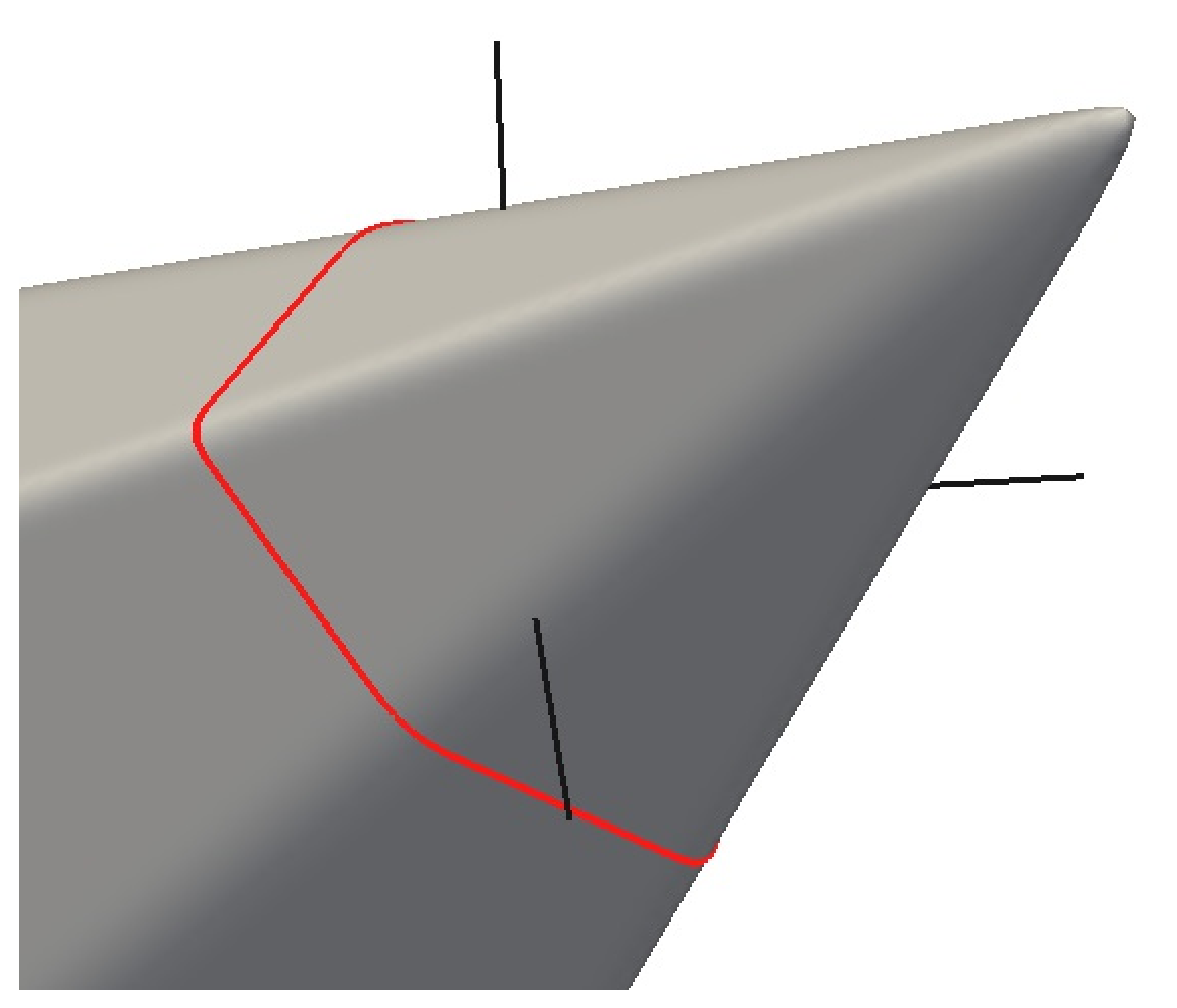
\includegraphics[width=6cm]{mc_octahedral_plane.eps} &
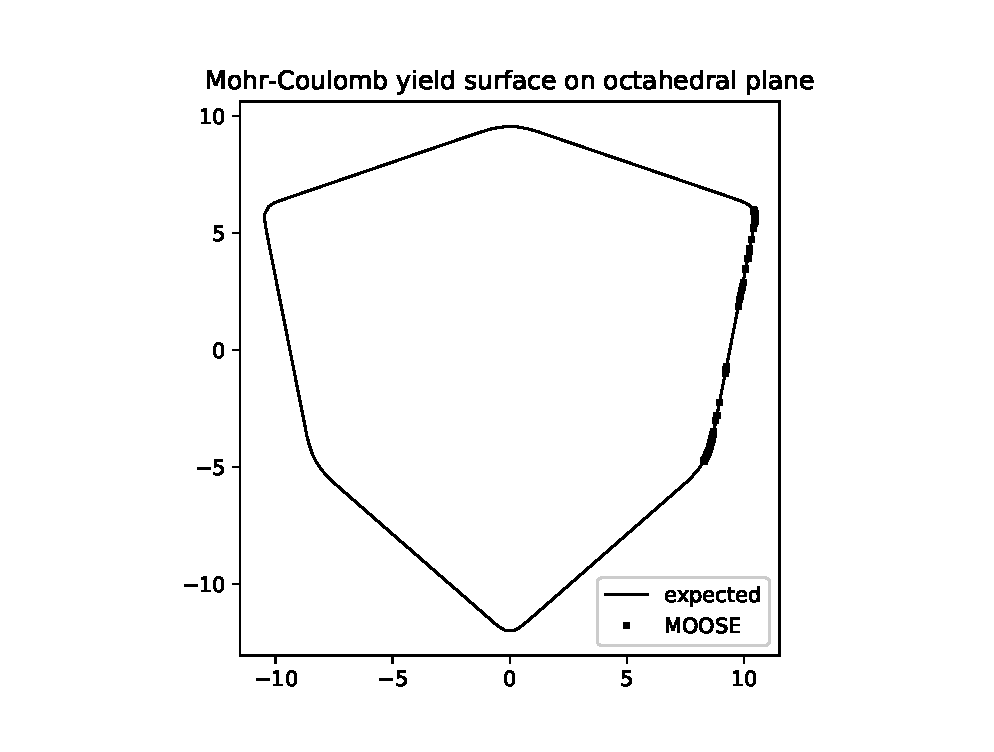
\includegraphics[width=8cm]{small_deform_21.eps}
\end{tabular}
\caption{Left: The tip of the Mohr-Coulomb yield surface.  This surface has
  $C=10$, $\phi=20^{\circ}$, and is smoothed with a smoothing
  parameter of 1.0.  The
  principal stress axes are shown in black.  The octahedral plane,
  where the mean stress is zero ($\tr\sigma=0$) is represented by the red line
  around the yield surface.  Right: The expected result
  is the hexagon, and the MOOSE results lie on the hexagon as
  desired.  Only the physical sextant ($\smax\geq\smid\geq\smin$) is
  sampled by MOOSE.}
\label{mc_octahedral_plane.fig}
\end{center}
\end{figure}


\section{The Mohr-Coulomb yield surface on the meridional plane}

Consider the two slices of the Mohr-Coulomb yield surface\footnote{An
  unusually large amount of smoothing has been used in this figure: I
  suggest in real situations the smoothing parameter be approximately
  $C/10$.} that are shown in Figure~\ref{mc.meridional.fig}.
Repeated deformations may be applied to a single element in order to
cause shear failure, and by recording the returned stresses, the yield
surface may be mapped out.  Figure~\ref{mc.meridional.fig} shows the results on the two
meridional planes, indicating that MOOSE's
Mohr-Coulomb yield functions are coded correctly.  The tests are {\tt
  small\_deform23} and {\tt small\_deform24}.

Looking carefully at the smoothed tip in
Figure~\ref{mc.meridional.fig}, the effect of the ordering of
the yield functions is evident: the lines do not intersect the
mean stress axis at precisely $90^{\circ}$.  Nevertheless, the
yield surface is provably convex, and the non-right intersection means
that MOOSE will stay away from the numerically troublesome regions
such as $\smax=\smid=\smin$.


\begin{figure}[htb]
  \begin{center}
    \begin{tabular}{ll}
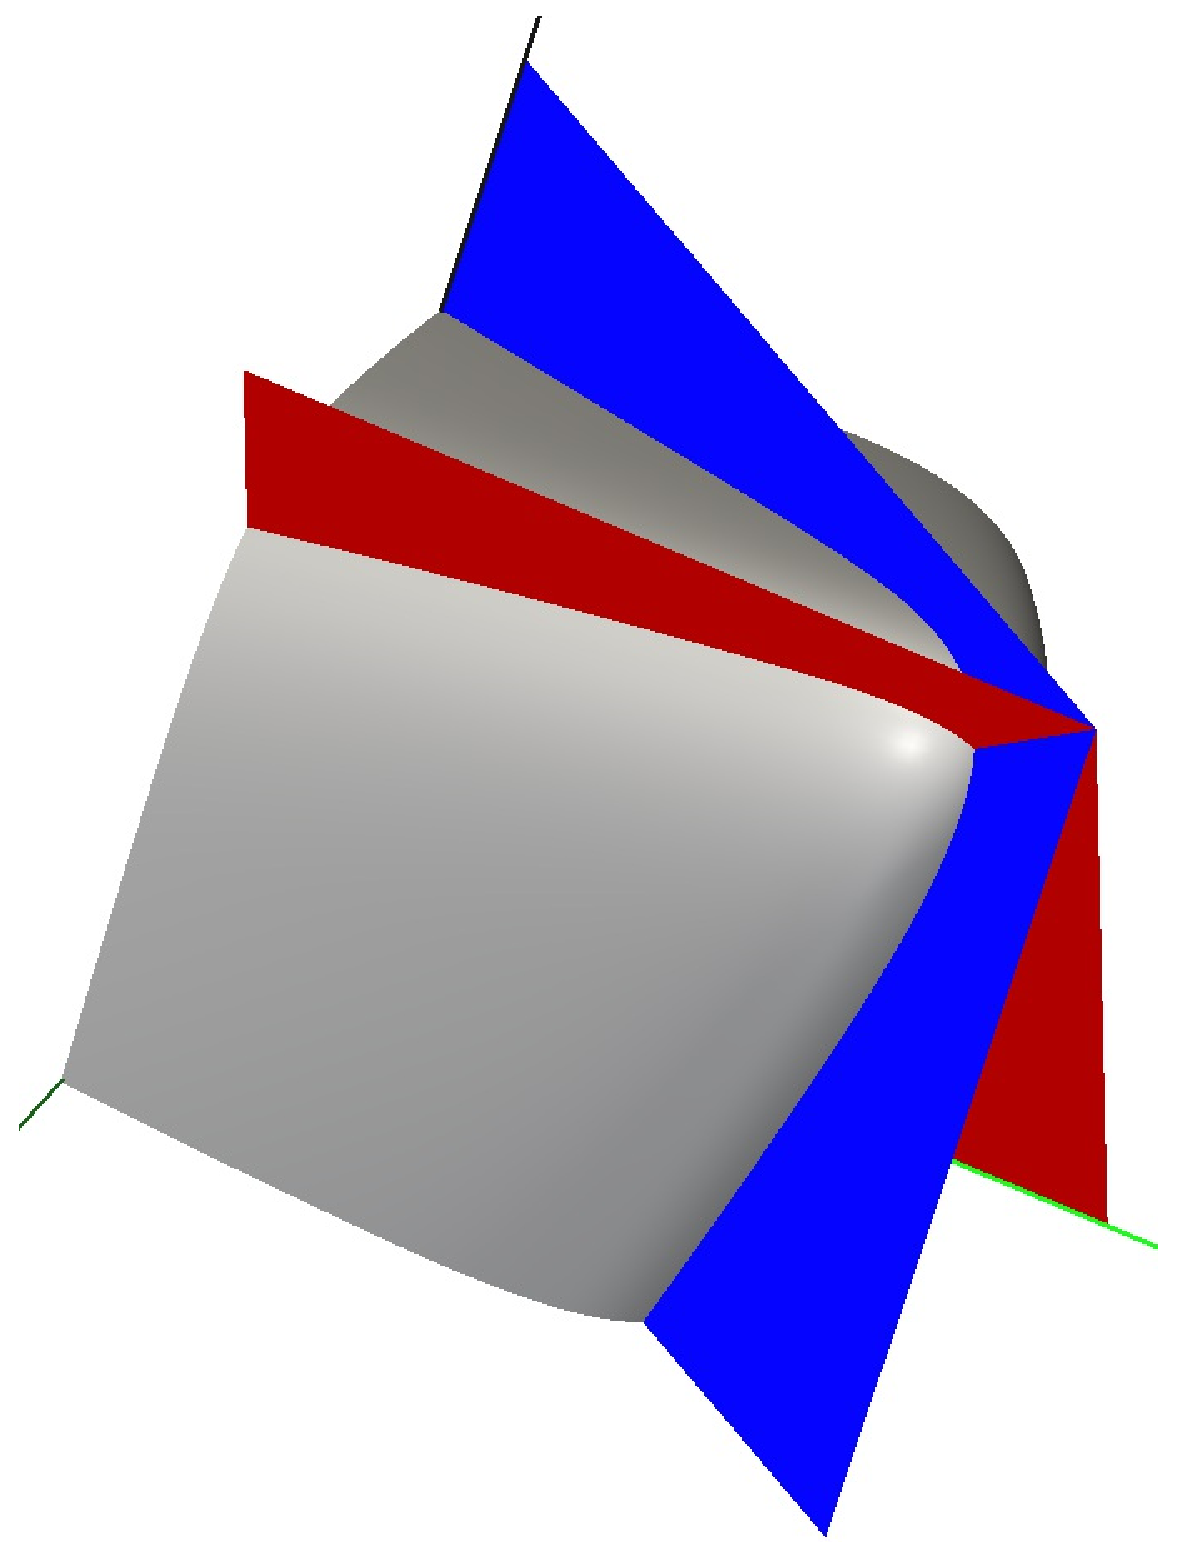
\includegraphics[width=6cm]{capped_mc_mc_with_planes.eps} &
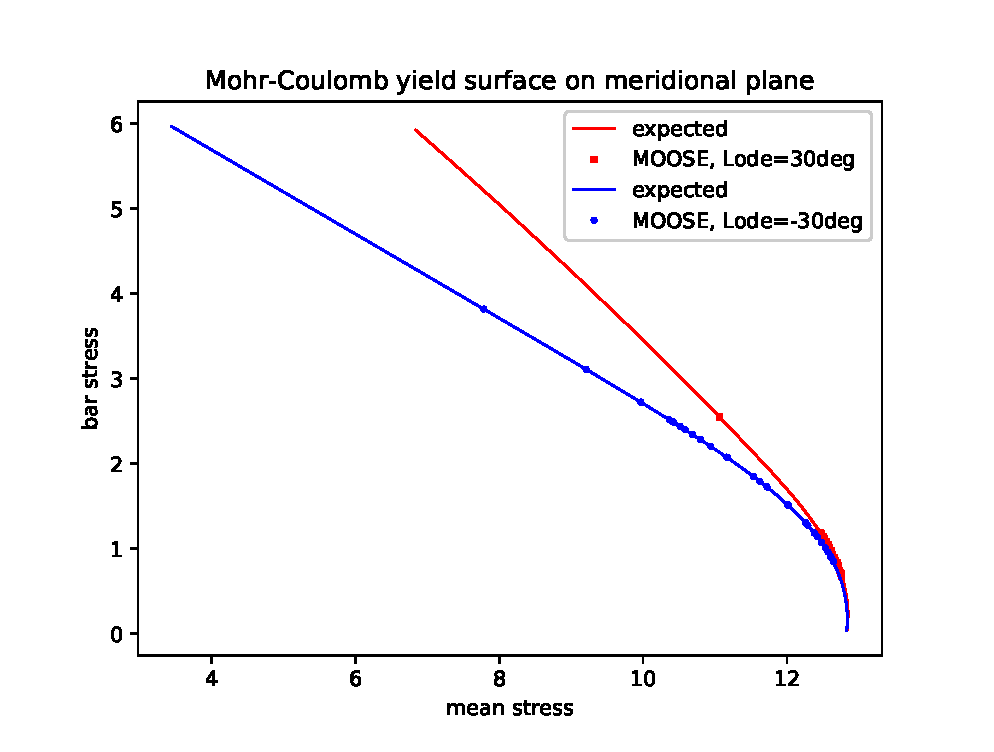
\includegraphics[width=8cm]{small_deform_23_24.eps}
\end{tabular}
\caption{Left: The tip of the Mohr-Coulomb yield surface.  This
  surface has $C=10$, $\phi=30^{\circ}$, and is smoothed with a
  smoothing parameter of 5.0.  The principal stress axes are shown in
  black ($\smax$), dark green ($\smid$) and light green ($\smin$).
  The wedge-shaped region defined by the planes is the physical region
  where $\smax\geq\smid\geq\smin$.  The blue plane is $\smid=\smin$,
  which is a Lode angle of $-30^{\circ}$.  The red plane is
  $\smax=\smid$, which is a Lode angle of $30^{\circ}$.  Right: The
  Mohr-Coulomb yield surface on the two meriodonal planes (blue and
  red).  The MOOSE results are shown as blue and red spots.  The axes
  are mean stress $ = \tr\sigma/3$ and bar stress
  $=\sqrt{s_{ij}s_{ij}/2}$, where $s_{ij}$ is the deviatoric part of
  the stress tensor.}
\label{mc.meridional.fig}
\end{center}
\end{figure}

\section{Hardening of the tensile and compressive strengths}

Both the tensile strength and the compressive strength may depend on
the internal parameter $i_{1}$.  Example cubic relationships are shown
in Figure~\ref{small_deform_hard_3_13.fig}.  The tests are {\tt
  small\_deform\_hard3} and {\tt small\_deform\_hard13}.

\begin{figure}[htb]
  \begin{center}
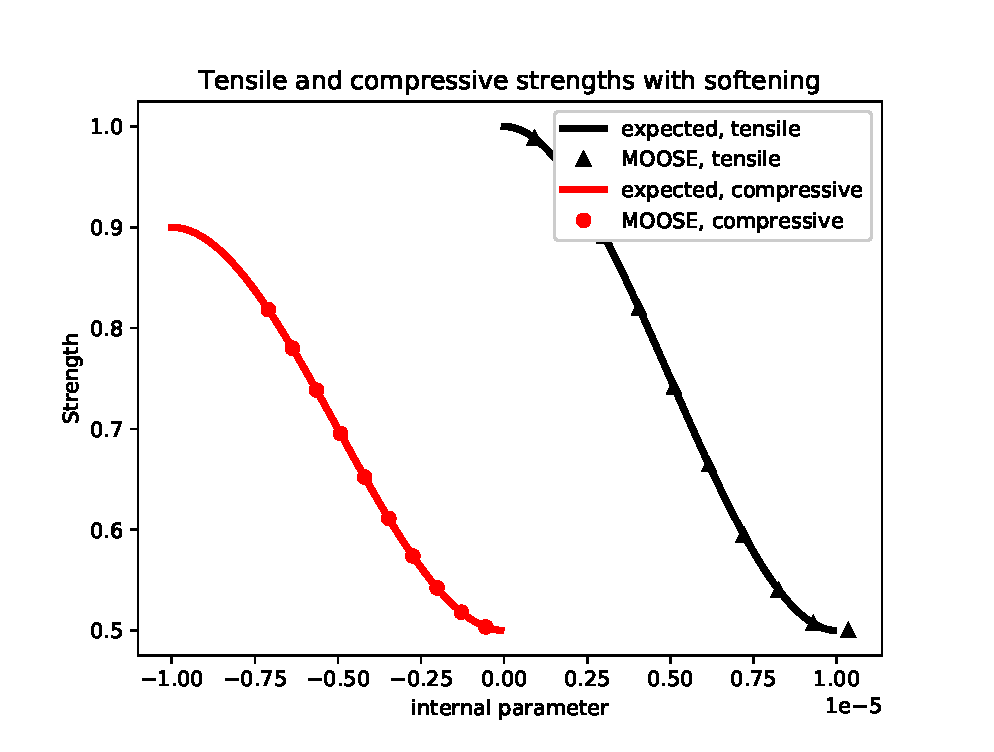
\includegraphics[width=8cm]{small_deform_hard_3_13.eps}
\caption{Examples of hardening of the tensile and compressive
  strengths, demonstrating that MOOSE produces the expected behaviour.}
\label{small_deform_hard_3_13.fig}
\end{center}
\end{figure}


\section{Hardening of the cohesion and friction angle}

Both the cohesion and friction angle may depend on
the internal parameter $i_{0}$.  Example cubic relationships are shown
in Figure~\ref{small_deform_hard_21.fig}.  The tests are {\tt
  small\_deform\_hard21} and {\tt small\_deform\_hard22}.

\begin{figure}[htb]
  \begin{center}
    \begin{tabular}{ll}
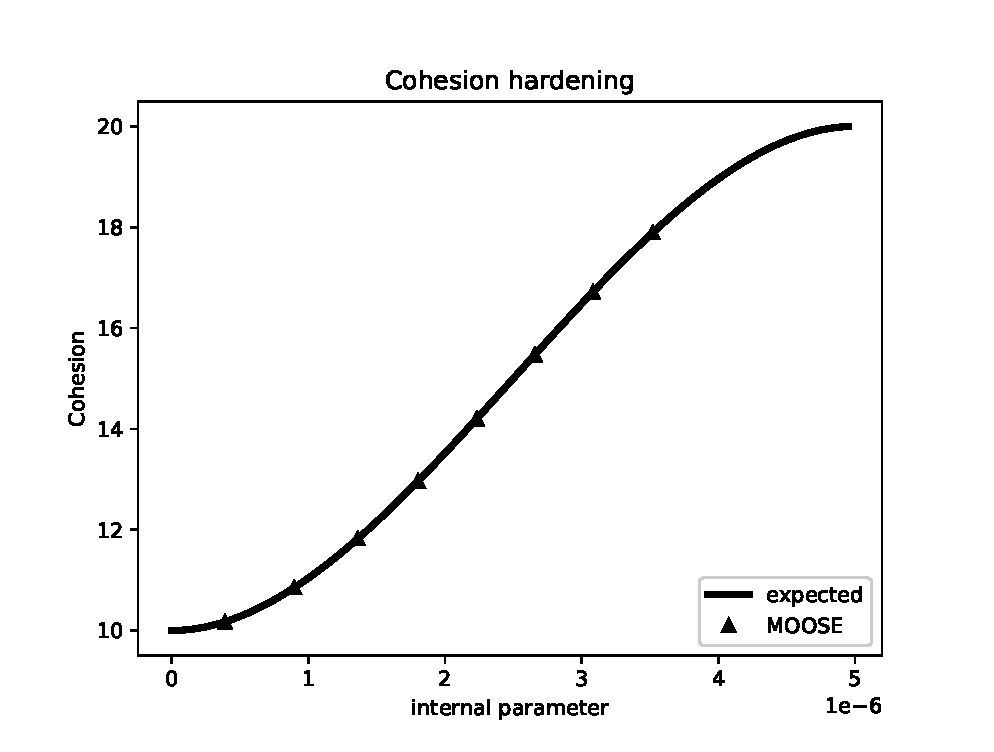
\includegraphics[width=6cm]{small_deform_hard_21.eps} &
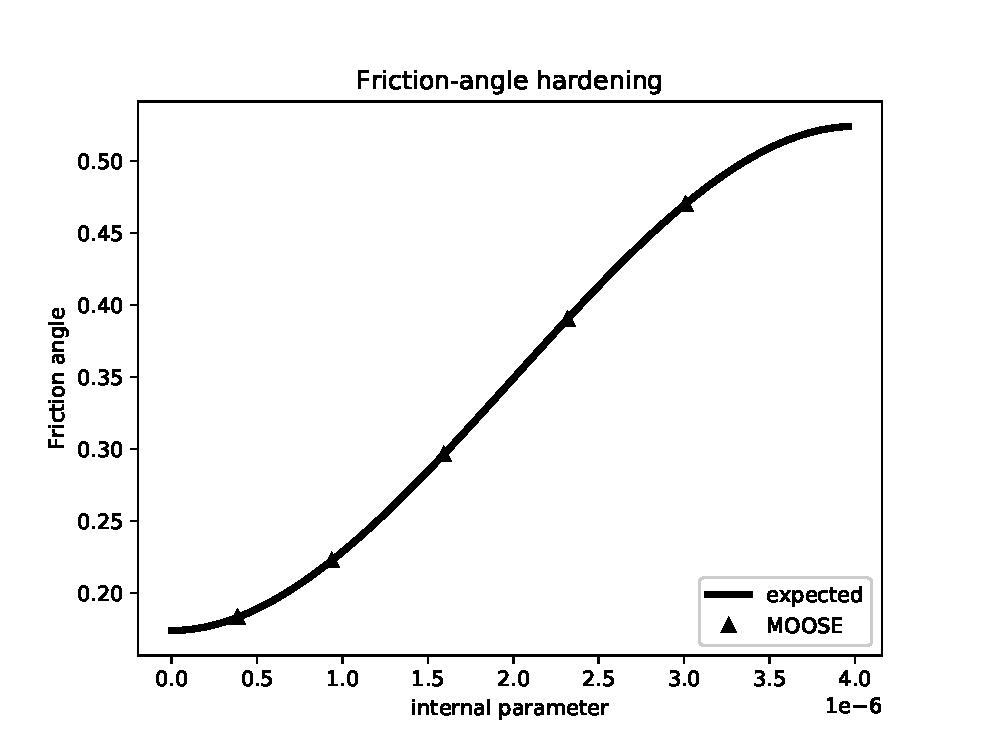
\includegraphics[width=6cm]{small_deform_hard_22.eps}
\end{tabular}
\caption{Examples of hardening of the cohesion and friction angle,
  demonstrating that MOOSE produces the expected behaviour.}
\label{small_deform_hard_21.fig}
\end{center}
\end{figure}

\section{Return to the yield surface from random positions}

Random displacements may be applied to a mesh in order to cause
failure in the elements, and the returned stresses may be recorded.
The test is {\tt random5}.  The results are shown in
Figure~\ref{random5.fig} where it is clear that MOOSE returns
correctly to the yield surface.

\begin{figure}[htb]
  \begin{center}
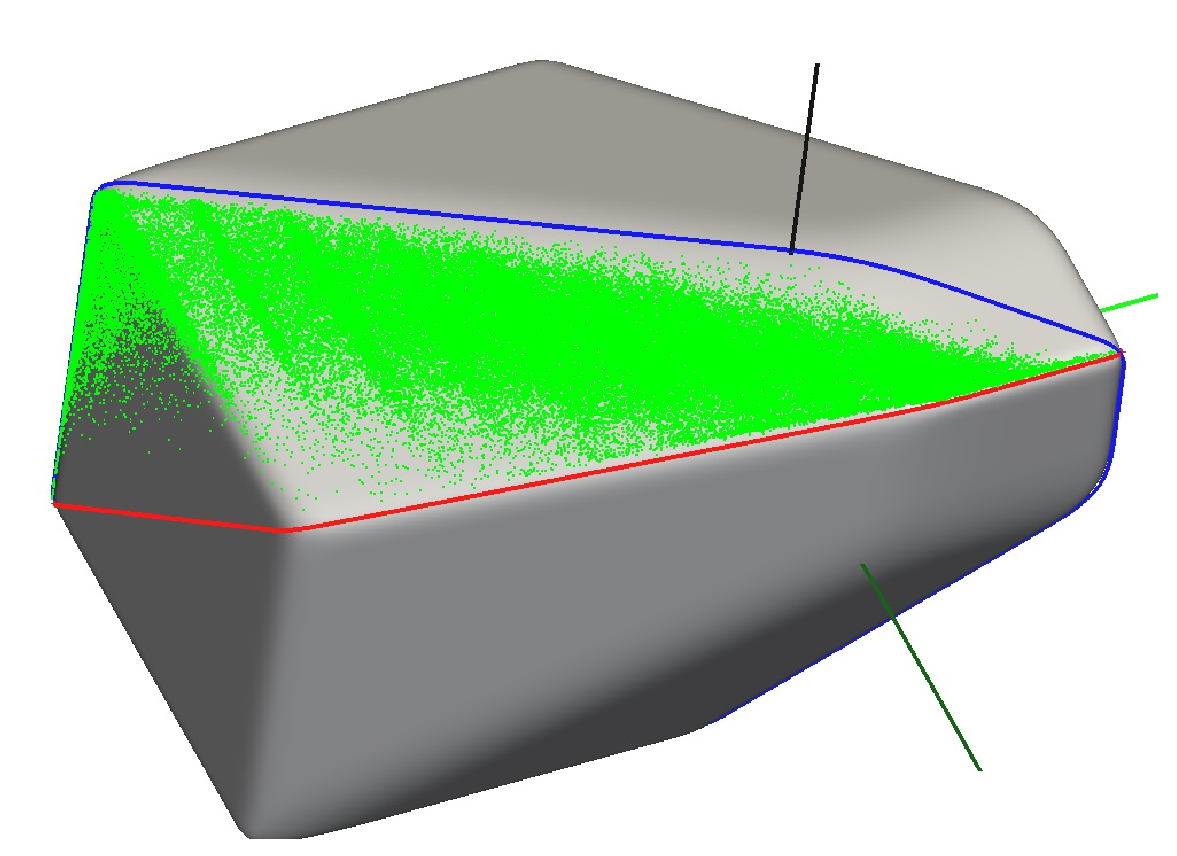
\includegraphics[width=8cm]{random5.eps}
\caption{Grey shape: the capped Mohr-Coulomb yield surface with
  $T=1.5$, $T_{c}=3$, $C=1$, $\phi=20^{\circ}$ and smoothing parameter
  of 0.2.  The other parameters are $\psi=3^{\circ}$ and Poisson's
  ratio $\nu=0.3$.  The principal stress axes are shown in black ($\smax$),
  dark green ($\smid$) and light green ($\smin$).  The plane defined
  by the red curve has $\smax=\smid$ (Lode angle of $30^{\circ}$), and
  the plane defined by the blue curve has $\smid=\smin$ (Lode angle of
  $-30^{\circ}$.  The physical region is the sextant lying between
  these curves.  Upon randomly deforming a mesh, the stresses in each
  element that experiences plastic deformation will lie on the yield
  surface.  The green dots are the results from 123400 applications of
  the return-map algorithm.  They lie on the yield surface as
  desired.}
\label{random5.fig}
\end{center}
\end{figure}




\end{document}

